\chapter{Radio packet format and retransmission scheme}\label{chap4}

The sensors communicate with a base station with a unidirectional radio link. There is no receiver module in the sensors. They can not have any kind of acknowledgement of their transmission, nor can they do carrier detection. The system has no means to verify whether a packet has been delivered successfully. Therefore, we design a retransmission scheme in order to improve event deliver rate. 

\section{Radio packet format and retransmission scheme}

In our design, each packet has 16-bit of payload plus one parity bit. Each packet is 64 milliseconds long, which is slightly less than 4 AC cycles (assuming 60Hz). Hence, we choose 4 AC cycles as a time slot for transmission. 

When a sensor detects an event, it transmits 5 packets in a timespan of 2.2 seconds. The event is successfully delivered when at least one packet is successfully received. In the rare case that another event detected on the same sensor before it finishes with the previous event, any further retransmissions of the previous event are abandoned. We call the previous event a \textit{flash event}. 

The sensor can detect zero-crossing of AC voltage, and use that to provide a 60Hz timer synchronous to AC cycles. All packet transmissions are synchronized to AC cycles. 

\begin{figure}[htb]
  \centering
  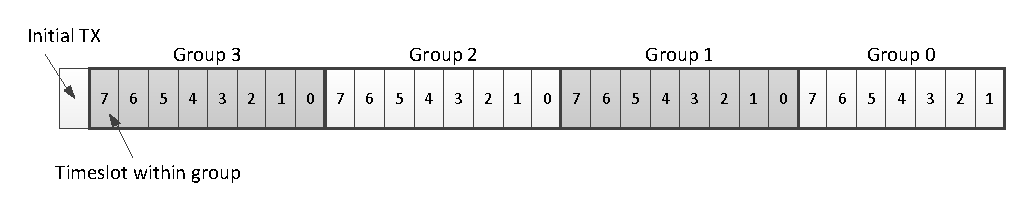
\includegraphics[width=\textwidth]{figures/slots}
  \caption[Transmission timeslots]{Transmission timeslots: There is an initial transmission, followed by 4 groups of timeslots. One slot is randomly picked from each group for a retransmission. }
  \label{fig:slots}
\end{figure}

When an event is detected, the sensor initiated a transmission at the next AC cycle. Following the initial time slot, there are 31 more slots, arranged in 4 groups. The groups have 8, 8, 8 and 7 time slots respectively. Fig.\ref{fig:slots} shows the arrangement of transmission time slots. The sensor randomly pick one slot from each group. Altogether there are 32 time slots, or 128 cycles, roughly 2.2 seconds. 

\begin{figure}[htb]
  \centering
  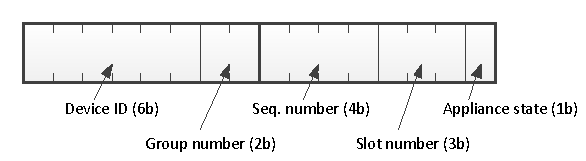
\includegraphics[width=0.8\textwidth]{figures/packet}
  \caption{16-bit packet format}
  \label{fig:packet}
\end{figure}

The format of each packet is shown in Fig.\ref{fig:packet}. The initial transmission of an event will have group number 0 and slot number 0. The group and slot number are included in the packet so that the receiver can estimate the delay from the event to the transmission. The 4-bit sequence number is advanced in every packet. The 6-bit device ID is hardcoded in every sensor node, allowing up to 64 sensors working in a same region with a single receiver. 

\section{Evaluation of the radio network}

The evaluation of our sensor network is presented in three parts. In simulation, we assume guaranteed delivery of packets as long as packets are not corrupted because of collision. In a controlled setup, we use an extra microcontroller to generate events, and the sensor nodes are placed close to the receiver. In the real setting, we deployed 20 sensors in our lab. The deployment will be discussed in detail in Chapter \ref{chap5}.

\subsection{Simulation: Poisson distribution events}

We developed the simulator program according to our packet format and retransmission scheme. We have a \textit{perfect packet delivery assumption}, which is: any packets that are not corrupted due to collision are to be successfully received. 

The test datasets are synthesized according to the following assumptions. 1) Appliances are independent with each other; 2) Events on appliance $A_k$ conform to a poisson distribution with parameter $\lambda_k$; 3) All appliances have the same poisson distribution parameter, i.e. $\lambda_k = \lambda$ for all $k$. Here $\lambda$ is the average number of events happend in 1 second with a single appliance. 

According to these assumptions, the overall events of all appliances conform to a poisson distribution with parameter $N\lambda$, where $N$ is the number of appliances. In another word, the density of events can be adjusted ether by adjusting $N$ or adjusting $\lambda$, ignoring flash events. Taking flash events into account, the result of high $N$ and high $\lambda$ are not exactly the same. In the case of high $\lambda$, there are more flash events, and they are more vulnerable to loss because they do not have all 5 transmission. In the case of high $N$, there are more chances of collision. 

In this simulation, we fix $N$ to be 6, and let $\lambda$ vary from $1/3$ to $1/20$, which means the expected interval between events on a same appliance is 3 to 20 seconds. Note that here $\lambda$ is much higher than what we expect in real settings. In real settings, appliances do not frequently change state in tens of seconds. We choose the numbers on purpose to stress our network. 



\subsection{Controlled experiments: Two-events collision test and Poisson distribution events}

\subsection{Evaluation in real settings}


